\documentclass{abntex2}
\usepackage[utf8]{inputenc}
\usepackage{graphicx}
\usepackage[num]{abntex2cite}

\titulo{Experimento 2: Regulador de tensão}
\autor{Lucas Rezende de Macedo - 14/0026363\\Jônatas Ribeiro Senna Pires - 14/0090983}
\data{9 de Abril de 2018}
\local{Brasília, Distrito Federal}

\begin{document}

\imprimircapa
\imprimirfolhaderosto

\tableofcontents
\listoffigures
\clearpage

\chapter{Experiências}

O procedimento experimental consiste na verificação do funcionamento dos circuitos retificadores representados pelas figuras \ref{fig:circuito1} e \ref{fig:circuito2}.

\begin{figure}[h]
  \centering
  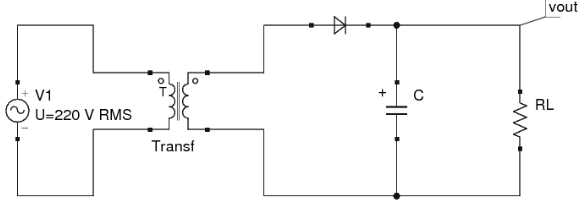
\includegraphics[scale = 0.7]{circuito1.png}
  \caption{Circuito retificador de meia onda montado no procedimento experimental.}
  \label{fig:circuito1}
\end{figure}

\begin{figure}[h]
  \centering
  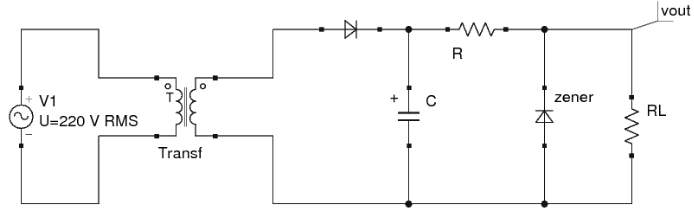
\includegraphics[scale = 0.7]{circuito2.png}
  \caption{Circuito retificador de meia onda com regulação de tensão por diodo zener montado no procedimento experimental.}
  \label{fig:circuito2}
\end{figure}

\section{Experiência 1}

Para a primeira montagem do circuito da figura \ref{fig:circuito1}, sem a carga ($R_L$), temos que a entrada ($v_I$) e saída no capacitor ($v_o$) são definidas conforme a figura \ref{fig:io1}.
\pagebreak

\begin{figure}[h]
  \centering
  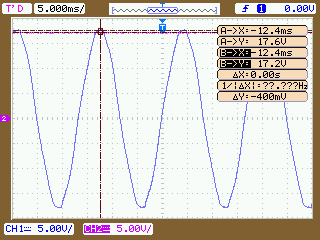
\includegraphics[scale = 0.7]{exp1-1.png}
  \caption{Gráfico da entrada (azul) e saída (rosa) do circuito da figura \ref{fig:circuito1} sem a carga ($R_L$).}
  \label{fig:io1}
\end{figure}

Para a segunda montagem do circuito da figura \ref{fig:circuito1}, com a carga ($R_L) = 2.17 k\Omega$, temos que a entrada ($v_I$) e saída no capacitor ($v_o$) são definidas conforme a figura \ref{fig:io2}.

\begin{figure}[h]
  \centering
  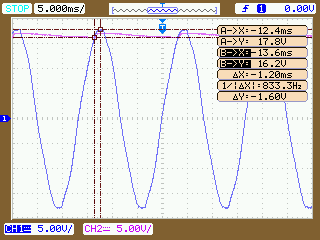
\includegraphics[scale = 0.7]{exp1-2.png}
  \caption{Gráfico da entrada (azul) e saída (rosa) do circuito da figura \ref{fig:circuito1} com a carga ($R_L$).}
  \label{fig:io2}
\end{figure}

\pagebreak
\section{Experiência 2}

Para o circuito da figura \ref{fig:circuito2}, realizamos a montagem com um resistor $R = 992.3\Omega$ com o capacitor $C = 1000\mu F$, $25V$. Para cada valor de resistência de carga ($R_L$) medimos os valores de tensão presentes na tabela \ref{tab:tensoes}.

Para obter a resistência de carga ($R_L = 492.15\Omega$) utilizamos dois resistores de resitência nominal $1k\Omega$ em paralelo. De forma análoga, para obter a resistência de carga ($R_L = 315.3\Omega$), utilizamos um resistor de $100\Omega$ e um de $220\Omega$ em série.

As tensões no capacitor e na carga para os valore de $R_L$ podem ser verificados nos gráficos das figuras \ref{fig:graf1} a \ref{fig:graf5}

\begin{table}[h]
\centering
\begin{tabular}{|l|l|l|l|l|}
\hline
$R_L(\Omega)$ & $V_{DC}$(V) & $V_{DC}(\infty) - V_{DC}(R_L)$ (V) & $V_{PP}^C$ (mV) & $V_{PP}^{R_L}$ (mV) \\
\hline
\infty        & 8,74      & 0                              & 146             & 10                  \\
\hline
2,17k         & 8,67      & 0,07                           & 150             & 10                  \\
\hline
985           & 8,33      & 0,41                           & 156             & 76                  \\
\hline
492,15        & 5,48      & 3,26                           & 206             & 66                  \\
\hline
315,3         & 3,96      & 4,78                           & 230             & 58                  \\
\hline
\end{tabular}
\label{tab:tensoes}
\caption{Tabela de valores de tensão para cada valor de $R_L$.}
\end{table}

\begin{figure}[h]
  \centering
  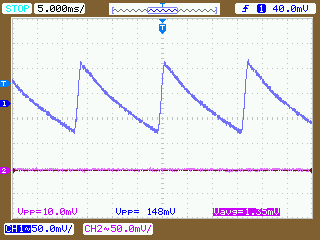
\includegraphics[scale = 0.7]{exp2-1.png}
  \caption{Gráfico da tensão no capacitor (azul) e na saída (rosa) do circuito da figura \ref{fig:circuito2} com a carga ($R_L = \infty$).}
  \label{fig:graf1}
\end{figure}

\begin{figure}[h]
  \centering
  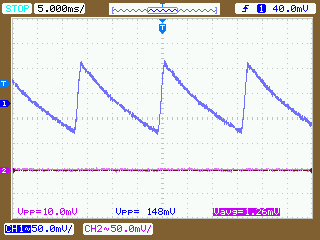
\includegraphics[scale = 0.7]{exp2-2.png}
  \caption{Gráfico da tensão no capacitor (azul) e na saída (rosa) do circuito da figura \ref{fig:circuito2} com a carga ($R_L = 2,17k\Omega$).}
  \label{fig:graf2}
\end{figure}

\begin{figure}[h]
  \centering
  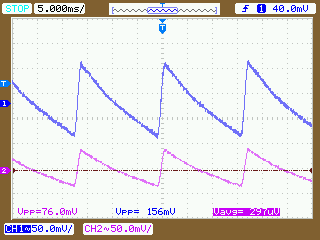
\includegraphics[scale = 0.7]{exp2-3.png}
  \caption{Gráfico da tensão no capacitor (azul) e na saída (rosa) do circuito da figura \ref{fig:circuito2} com a carga ($R_L = 985\Omega$).}
  \label{fig:graf3}
\end{figure}

\begin{figure}[h]
  \centering
  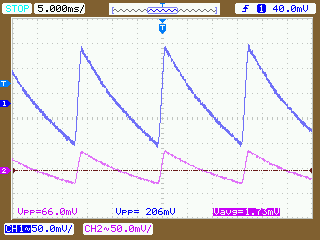
\includegraphics[scale = 0.7]{exp2-4.png}
  \caption{Gráfico da tensão no capacitor (azul) e na saída (rosa) do circuito da figura \ref{fig:circuito2} com a carga ($R_L = 492.15\Omega$).}
  \label{fig:graf4}
\end{figure}

\begin{figure}[h]
  \centering
  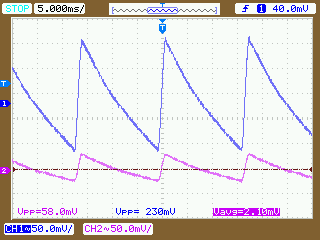
\includegraphics[scale = 0.7]{exp2-5.png}
  \caption{Gráfico da tensão no capacitor (azul) e na saída (rosa) do circuito da figura \ref{fig:circuito2} com a carga ($R_L = 315.3\Omega$).}
  \label{fig:graf5}
\end{figure}
\pagebreak
\chapter{Discussão}

\section{Questão 1 - Comportamento com a redução de $R_L$}
Para o circuito \ref{fig:circuitos}(a), um diodo ideal se comporta como um circuito aberto quando está inversamente polarizado, impedindo a passagem de corrente, zerando a saída. E o diodo se comporta como um curto circuito quando está diretamente polarizado,
permitindo, instantâneamente, que toda a corrente disponível passe pelo dispositivo, copiando a entrada na saída, assim como mostrado em vermelho na figura \ref{fig:comp1}.

\begin{figure}[h]
  \centering
  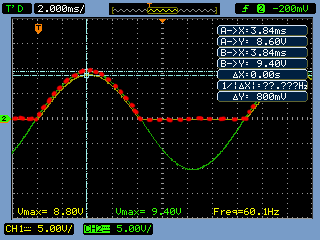
\includegraphics[scale = .7]{circuito-1a-esboco.png}
  \caption{Esboço do comportamento esperado para um diodo ideal para o circuito 1.}
  \label{fig:comp1}
\end{figure}
\pagebreak
O resultado obtido no experimento é muito similar ao do diodo ideal, com pequenas diferenças nos momentos em que o diodo está diretamente polarizado, visto que o diodo real tem um comportamento exponencial somado a uma queda de tensão no dispositivo.
Ao compararmos com o modelo de queda de tensão constante, podemos perceber que o comportamento é mais semelhante ao do diodo real, visto que considera a queda de tensão no dispositivo, mas com diferenças pois não considera o comportamento exponencial.

\\Para o circuito \ref{fig:circuitos}(b), considerando diodos ideais, não teríamos o comportamento limitante, mas sim a saída sempre em 0 V, visto que sempre haveria um curto circuito entre Vs e o nó de referêcia (relacionando com o modelo de queda de tensão constante, teríamos Vd = 0 V, limitando sempre em 0). Comportamento demonstrado em vermelho na figura \ref{fig:comp2}.

\begin{figure}[h]
  \centering
  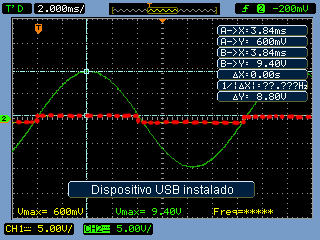
\includegraphics[scale = .7]{circuito-1b-esboco.png}
  \caption{Esboço do comportamento esperado para um diodo ideal.}
  \label{fig:comp2}
\end{figure}

\\Entretanto, considerando o modelo de queda de tensão constante, um dos diodos limitaria a tensão em 1,1 V instantâneamente no regime positivo da fonte de tensão quando diretamente polarizado e o outro diodo limitaria instantâneamente em -1,1 V no regime negativo da
fonte de tensão (quando este diodo estaria diretamente polarizado). Comportamento muito próximo do obtido experimentalmente, apenas não levando em consideração a curva exponencial durante a troca de regime da fonte de tensão e pequenas variações em Vd.

% \pagebreak

Para o circuito \ref{fig:circuitos}(c), se considerarmos o modelo de queda de tensão constante o modelo ideal de diodo zener, temos que quando o dispositivo está diretamente polarizado o circuito limita a saída em -Vd e quando está inversamente polarizado o circuito limata Vs em Vz. Assim como mostrado em vermelho na figura \ref{fig:comp3}.

\begin{figure}[h]
  \centering
  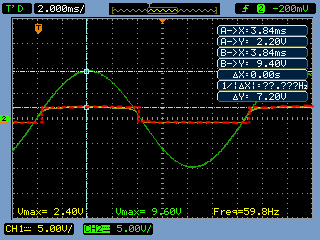
\includegraphics[scale = .7]{circuito-1c-esboco.png}
  \caption{Esboço do comportamento esperado para um diodo ideal.}
  \label{fig:comp3}
\end{figure}
\pagebreak
O comportamento do diodo real em relação ao ideal é muito similar, apenas não considerando a curva exponencial na troca de regime e pequenas variações em Vd e Vz.
Se o diodo Zener ideal possuísse um comportamento semelhar ao diodo ideal, teríamos apenas um curto circuito para qualquer regime da fonte de tensão.

\\Para o circuito \ref{fig:circuitos}(d), considerando o modelo de queda de tensão constante como o modelo ideal, temos o comportamento mostrado em vermelho na figura \ref{fig:comp4}.
Um dos diodos limita a tensão em Vz durante o regime positivo da fonte e o outro diodo limita em -Vz durante o regime negativo da fonte.

\begin{figure}[h]
  \centering
  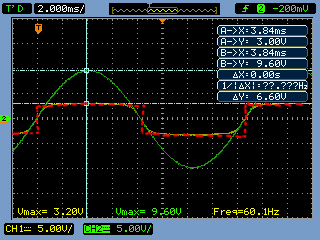
\includegraphics[scale = .7]{circuito-1d-esboco.png}
  \caption{Esboço do comportamento esperado para um diodo ideal.}
  \label{fig:comp4}
\end{figure}

O comportamento do diodo real em relação ao ideal é muito similar, apenas não considerando a curva exponencial na troca de regime e pequenas variações em Vz.
Se o diodo Zener ideal possuísse um comportamento semelhar ao diodo ideal, teríamos apenas um curto circuito para qualquer regime da fonte de tensão.

\section{Questão 2 - Comportamento com retificador de onda completa}

% O periodo de ripple eh menor pq a frequencia dobra e o ripple diminui

O circuito retificador tem esse nome dado que para uma tensão menor que sua tensão de polarização direta ($V_d$), a saída torna-se uma tensão contínua, como podemos ver na figura \ref{fig:retificador}, no caso do circuito da figura \ref{fig:circuitos}(a) essa tensão de saída é 0.

O circuito limitador tem esse nome porque ele faz com que a tensão máxima que o circuito possa atingir seja seu $V_d$, como podemos ver na figura \ref{fig:limitador}.

\begin{figure}[h]
  \centering
  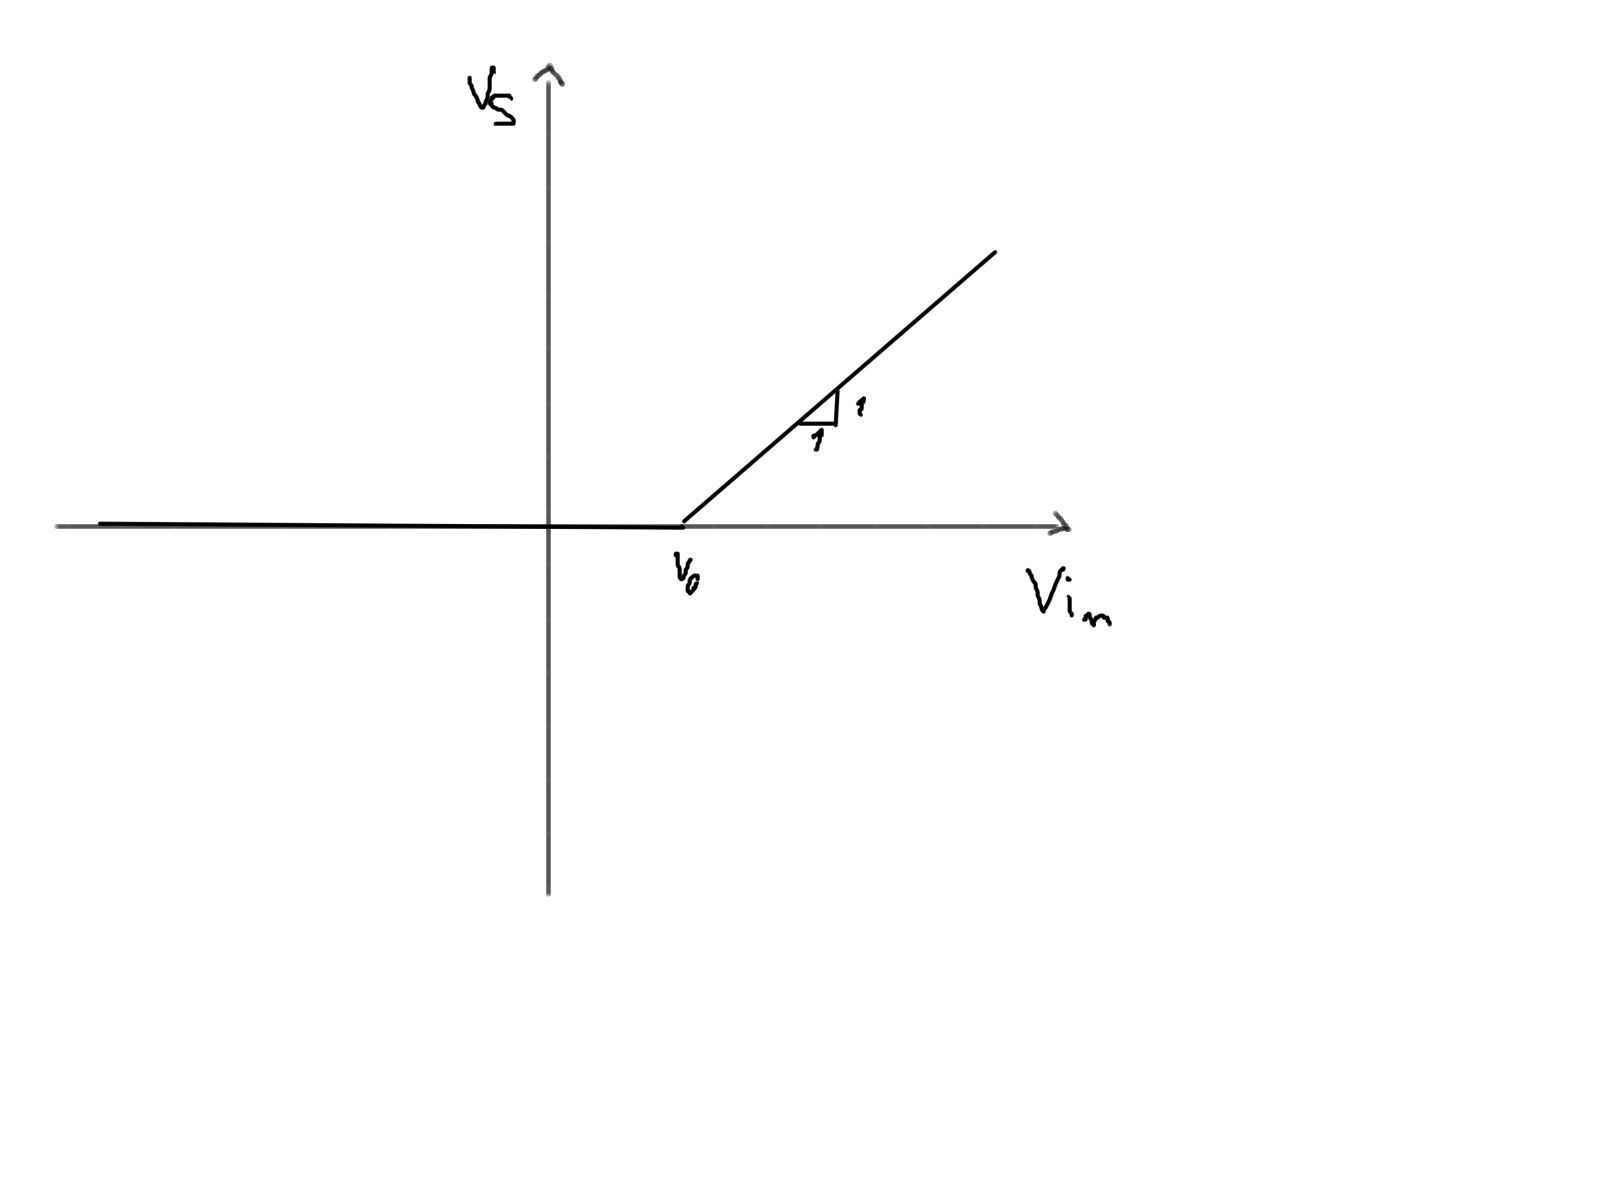
\includegraphics[scale = 0.2]{grafRetificador.jpeg}
  \caption{Gráfico da característica de transferência de um circuito retificador.}
  \label{fig:retificador}
\end{figure}

\begin{figure}[h]
  \centering
  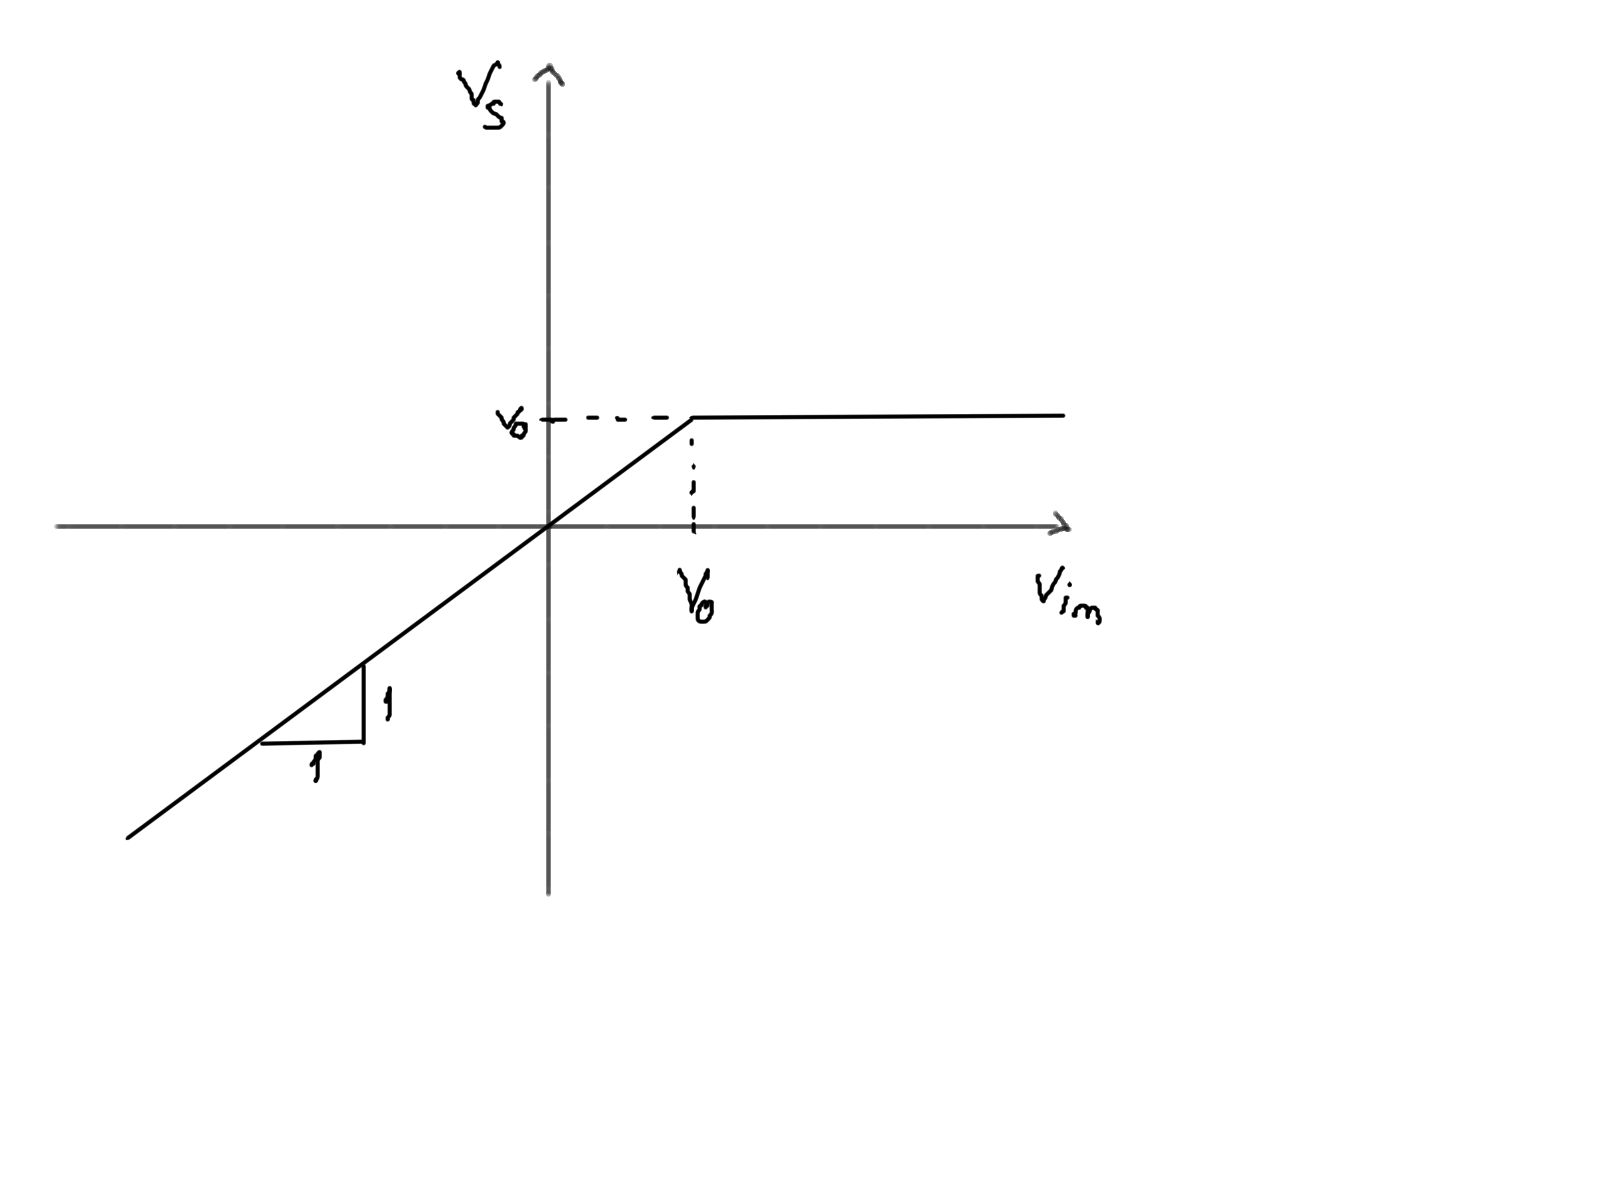
\includegraphics[scale = 0.75]{grafLimitador.jpg}
  \caption{Gráfico da característica de transferência de um circuito limitador.}
  \label{fig:limitador}
\end{figure}

Os circuitos da figura \ref{fig:circuitos} com exceção do circuito (a) podem ser considerados limitadores por reduzirem a amplitude da onda de saída ao valor da tensão de polarização direta ou de ruptura dos diodos do circuito.

\section*{Referências}


[1] SEDRA, Adel S.; SMITH, Kenneth Carless. Microelectronic circuits. New York: Oxford University Press, 1998.

[2] RAZAVI, Behzad; BEHZAD, Razavi. RF microelectronics. New Jersey: Prentice Hall, 1998.

\end{document}
